\subsection*{Source Coding}
\textbf{Information:}

Mesure de l'incertitude ou du désordre d'un système. Plus il y a
d'incertitude, plus il y a d'information. L'information se mesure en bits.

\underline{La mesure d'information:}

apportée par un évenement: $I(E) = -\log_2(P(E))[\text{bits}]$.

\textbf{Entropy:}

Quantité moyenne d'information contenue dans un message. Elle dépend
de la probabilité des symboles du message et de leur indépendance. L'entropie maximale
est atteinte quand tous les symboles sont équiprobables et indépendants.

\underline{La moyenne de l'information:}

(ou hentropie) $H$ envoyée par une source $S$ de $n$ symboles
$X_i$ avec une probabilité $p_i$ est:
$H(S) = -\sum_{i=1}^{n}p_i\cdot\log_2(P(X_i))[\text{bits}]$.

\textbf{Huffman Coding:}

Algorithme qui permet de compresser des données en utilisant
un code binaire variable, adapté à la fréquence d'apparition des symboles.

\setlength{\intextsep}{-5pt}
\begin{wrapfigure}{r}{0.3\textwidth}
    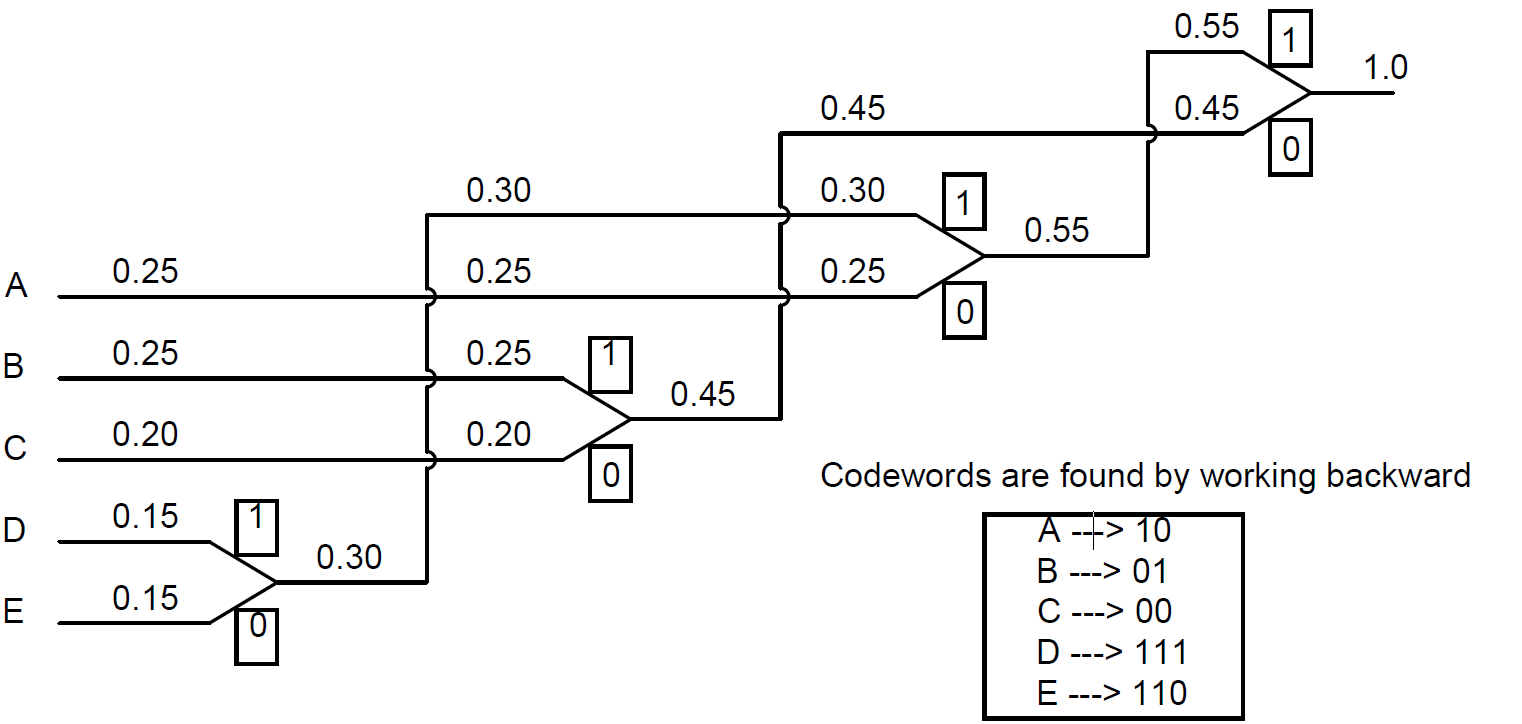
\includegraphics[width=\linewidth]{images/arbre_huffman.png}
\end{wrapfigure}
\underline{Construction de l'arbre de Huffman:}

Extraire les deux nœuds de plus faible
priorité de la file, les fusionner en un nouveau nœud dont la fréquence est la somme
des deux, et l'insérer dans la file, jusqu'à ce qu'il ne reste qu'un seul nœud dans
la file, qui est la racine de l'arbre.

\textbf{Lempel-Ziv Coding:}

Algorithme de compression sans perte qui utilise un
dictionnaire dynamique pour coder les données. Le principe est de remplacer les
séquences répétées par des références au dictionnaire.

\underline{L'algorithme de Lempel-Ziv}:

Chaque mot du dictionnaire va être séparé entre
un préfixe et son dernier bit, au lieu de transmettre le préfixe, on va transmettre
son numéro d'apparition dans le dictionnaire (sous forme binaire) plus le dernier
bit qui sera appelé bit d'innovation. $S = 000101110010100101$
\setlength{\intextsep}{0pt}
\begin{figure}[H]
    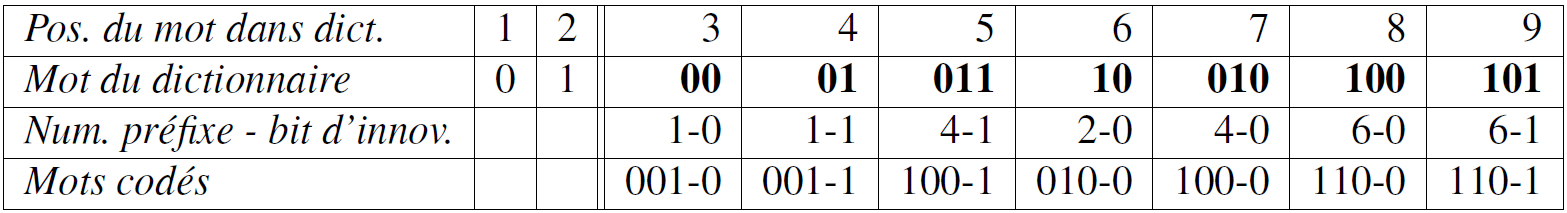
\includegraphics[width=\linewidth]{images/lempel-ziv_table.png}
\end{figure}

\underline{Taille moyenne d'un code:}

envoyé par une source utilisant $l_i$ bits pour chaque symboles :
$\overline{L}=\sum_{i=1}^{n}p_i\cdot l_i[\text{bits par symboles}]$.

\underline{Efficacité d'un code:}

$\text{eff}=\frac{H(S)}{\overline{L}}$.



